\documentclass[12pt]{article}

\usepackage[a4paper, total={6in, 9in}]{geometry}
\usepackage{booktabs}
\usepackage{adjustbox}
\usepackage{tikz}
\usepackage{gensymb}
\usepackage{float}
\usepackage{graphicx}
\usepackage{hyperref}
\usepackage{csvsimple}
\usepackage[toc,page]{appendix}
\usetikzlibrary{shapes, arrows}
\graphicspath{ {./images/} }


% Figure Setup
\tikzstyle{boxes} = [rectangle, minimum width=4cm, minimum height=1cm, text centered, text
width=3cm, draw=black]

\tikzstyle{meshOrCloud} = [cloud, minimum width=2cm, minimum height=1cm, text centered, text
width=3cm, draw=black, cloud puffs=12, cloud puff arc=150, aspect=2]

\tikzstyle{diamond} = [diamond, minimum width=2cm, minimum height=1cm, text centred, text
width=2cm, draw=black]

% Database Defn
\makeatletter
\tikzset{
    database/.style={
        path picture={
            \draw (0, 1.5*\database@segmentheight) circle [x radius=\database@radius,y radius=\database@aspectratio*\database@radius];
            \draw (-\database@radius, 0.5*\database@segmentheight) arc [start angle=180,end angle=360,x radius=\database@radius, y radius=\database@aspectratio*\database@radius];
            \draw (-\database@radius,-0.5*\database@segmentheight) arc [start angle=180,end angle=360,x radius=\database@radius, y radius=\database@aspectratio*\database@radius];
            \draw (-\database@radius,1.5*\database@segmentheight) -- ++(0,-3*\database@segmentheight) arc [start angle=180,end angle=360,x radius=\database@radius, y radius=\database@aspectratio*\database@radius] -- ++(0,3*\database@segmentheight);
        },
        minimum width=2*\database@radius + \pgflinewidth,
        minimum height=3*\database@segmentheight + 2*\database@aspectratio*\database@radius + \pgflinewidth,
    },
    database segment height/.store in=\database@segmentheight,
    database radius/.store in=\database@radius,
    database aspect ratio/.store in=\database@aspectratio,
    database segment height=0.1cm,
    database radius=0.25cm,
    database aspect ratio=0.35,
}
\makeatother

\tikzstyle{line} = [thick, -, >=stealth]
\tikzstyle{arrow} = [thick, ->, >=stealth]

\author{Josiah Craw\\35046080}

\title{\huge{Affordable in home internet of things temperature sensor}}

\begin{document}

\maketitle

\newpage

\section*{Abstract}

\newpage

\tableofcontents

\newpage

\section{Introduction}
The project is the design of a internet of things (IoT) temperature sensor. The intent of this
product is to enable home renters to collect accurate temperature data as evidence that a home may
be too cold in the winter. The solution must be low cost, have enough storage for a month of data
collections and must be small and easy to hide in a home. 

The internet of things is a concept where devices are internet connected to allow remote control
or remote data collation and management. These systems can provide modern convenience to many
different parts of the home, such as in smart lighting. This space has become very popular in the
last several years, with large companies such as Nest and Ring designing intelligent internet of
things products. These companies has been bought by Google and Amazon, this demonstrates the
consumer's and industry's demand for a smarter home.

Over the last few years, several different technologies have emerged to accommodate this market,
the first is ZigBee, an open licence project using the IEEE 802.15.4 standard for mesh networks.
This technology has been widely adopted by the internet of things industry and is used in products
like Phillips Hue lighting. The second major technology used in this field is Bluetooth, with
recent versions of Bluetooth the energy consumption of these devices has been reduced this is
Bluetooth low energy (BLE). Also, recently Bluetooth supports mesh networking, making it good for
use in smart home and IoT applications.

\section{Requirements}
The main requirements for this project are that the design must be low cost and last between two
and four weeks for both data collection and battery usage. The device should be able to connect to
the internet, allowing the data to be accessed remotely as well as allowing the sensors to offload
data to external storage.

\subsection{RF Connectivity}
The system should include some form of internet connection interface to allow the data to be put 
into a cloud storage system. A form of wireless communication between the modules and a phone,
this could either be implemented with all modules communicating to each other and having a master
node that connects to the users device or with every node connecting to the users device
separately. 

\subsubsection{Zigbee vs WiFi vs Bluetooth Low Energy}
The main competitors in the RF connectivity space is Zigbee, WiFi, and Bluetooth low energy.
ZigBee is based on the IEEE 802.15.4 standard, this technology allows low power mesh network 
transmission at 2.4GHz frequency. This connectivity system is widely used in the IoT industry with
standards such as light link being used to connect smart lighting products by manufactures like
Phillips and Xiaomi. The next technology is WiFi the advantages of WiFi is the ability to use it
to seamlessly access the wider internet, however the system is complicated as each unit would have
to be completely independent, with each sensor in the network connecting directly to the users
private network. WiFi is also uses a significant amount of power. Finally Bluetooth Low Energy
(BLE) is power efficent, and can also connect directly to a users phone or computer with Bluetooth
compatability.

\subsection{Data Collection}
Data collection is an important part of the sensor as the hardware must be able to store between
two and four weeks to meet the specifications. All data collected will need to contain the sensor
data, as well as a time component, this time component will most likely have to be sourced from a
real time clock (RTC) as the specifications require operation even when internet is unavailable.
This amount of data will most likely require some external storage in the form of EEPROM,
electronically erasable read only memory. This data when offloaded into the cloud will need to be
kept secure to avoid user data breaches. Different database and storage solutions will need to be
considered for the cloud storage aspect of the solution.

\subsection{Power Consumption}
For this project the power use is very important as the system should be able to seamlessly
record data for a complete two to four week period. This means that keeping power consumption is
important in the success of the design.

\section{Hardware}
The chosen final specifications for the design were chosen to meet the requirements, focusing on
the simple usability of the design as well as keeping the power consumption low enough so the
device may run uninterrupted.

\subsection{Processor}
The chosen processor is from ST Microelectronics, specifically the STM32WB55CEU6. This MCU was 
chosen as it integrates both ZigBee and BLE support on one chip. This has two benefits, the first 
is cost as the unit integrates both the MCU and the transmit/receive functionality the cost is 
reduced as only one relativity affordable chip is required, with the chip costing \$6.65 for a 
single unit and \$3.76 each in 1,000 quantity all in USD.

This chip also has advantages for power consumption, as the package consists of two separate Arm
cortex processors. The first is a Cortex M4 this is dedicated to running the application and is a
very low energy part. The second is a Cortex M0+ this is dedicated to running the communication
stack. The network stack in this processor is capable of calling interrupts, this means that the
the low power M4 processor can be put into deep sleep mode to conserve power and can be woken by a
central node over the network to process the current temperature then send it over the network
before returning to deep sleep. 

\subsection{Temperature Sensor}

\subsection{Power Delivery}
The main module has a simple 3.3V regulator, this part is built into the main data collection and
ZigBee board. This keeps the auxiliary more simple, keeping manufacturing costs low as auxiliary
modules have smaller production than the ZigBee/data collection board. As the STM microcontroller
and temperature sensor operate at 3.3V V\textsubscript{DD} for the board is at 3.3V. For potential
expansion boards an external regulator can be used on board to supply required voltages before
feeding into the main board. 

Due to the variability of the design the power delivery is done on the auxiliary modules, this
means this if a unit, such as the base station is designed to powered externally as it is expected
to always be online. Where as batteries can be attached to make the design portable within the
home.

\subsection{Modules}
The design is to be modular to keep the production costs low as the entire system will have a low
initial production run of 5,000 units and to keep the PCB and component assembly cost as low as
possible each the main unit containing the STM MCU and the temperature will feature a six pin
connector with Voltage in, voltage out, ground and USART as well as one GPIO pins for future 
expansion. These pins will interface with external battery pack or base station modules.

\subsubsection{Data Collection Board}
The data collection board is design to contain the STM processor as well as the temperature 
sensor. Alongside these two the board contains supporting peripherals such as power delivery
components and the PCB antenna, with the required components. The PCB antenna is used to keep the
unit affordable as extra costly external components are not required.

The 3D render of the board shown in Figure {\ref{fig:3dpcb}}. This render shows how compact the
board is. It was determined that the board should be small to allow for greater options in future
expansion. As 3D footprints were not availble for all components some appear as coloured boxes,
some such as the microprocessor were made manually to aid visual representation.

\begin{figure}[H]
\includegraphics[width=\textwidth]{3D-PCB}
\caption{3D CAD layout of the data collection board}
\label{fig:3dpcb}
\end{figure}

The PCB and schematic layouts shown below show that most of the components are used for power
delivery to the microprocessor. Specifically, some of the power delivery shown in Figure
{\ref{fig:mainsch}} as C17, C18 and L1 allow the processor to run in SMPS mode, this allows the
processor to run in a lower power mode if V\textsubscript{DD} is high enough, around 2.0V or
above. The schematic also shows the two different oscillators, with one operating at 32MHz and the
other at 32.768kHz. The former is used for the RF and system clock and the latter is used bu the
real time clock.

\begin{figure}[H]
\includegraphics[width=\textwidth]{main-sch}
\caption{Schematic of data collection board}
\label{fig:mainsch}
\end{figure}

Finally below in Figure {\ref{fig:mainbrd}} is the PCB layout for the data collection board. As
shown in this image there are cut outs in the ground plane, this first of which is under the
antenna this is a requirement for the antenna layout given by STM in the application guides. The
next ground plane cut out is under the temperature sensor, this has been done to thermally isolate
the temperature sensor as many components dissipate heat on to the ground plane. Also shown are
several vias to the ground plane, these were placed to reduce the distance to ground for many
components, for parts such as decoupling capacitors this is very important as it reduces noise in
the system.

\begin{figure}[H]
\includegraphics[width=\textwidth]{ZigBee-Board}
\caption{PCB layout of the data collection board}
\label{fig:mainbrd}
\end{figure}

\subsubsection{Battery Expansion Board}
The battery board contains holder for two 18650 size lithium ion batteries, these batteries
contain enough power to keep the data collection board operating for 4 weeks. The rest of the
spare GPIO is routed out to five pins, with the GPIO, two USART and voltage out and the ground.
This will allow the system it potentially allow other sensors to be added to the unit. The layout
of this board is shown in Figure {\ref{fig:batbrd}}.

\begin{figure}[H]
\includegraphics[width=\textwidth]{battery-brd}
\caption{PCB layout to the battery expansion board}
\label{fig:batbrd}
\end{figure}

As shown in the figure above the board is keep as simple as possible, this is in an effort to
keep the assembly and part costs down. 

\subsubsection{Base Station Expansion Board}
This module is much more complicated than the battery board, this board uses a DC barrel jack to
power it from the main supply. This board also contains an ESP32 module this module is integrated
for the base station to allow WiFi connectivity. There is also EEPROM to allow for long term data
storage on the board. The ESP32 is connected to the USART connections of the STM micro 
controller, in this configuration the STM will be running in a slave like manner, with is being 
used primarily as a transmitter for into the ZigBee network. The ESP32 will be running Amazon 
FreeRTOS this is based on the popular FreeRTOS platform. The schematic PCB layout for the base 
station expansion board is shown below in Figures {\ref{fig:basesch}} and {\ref{fig:basebrd}}.

\begin{figure}[H]
\includegraphics[width=\textwidth]{base-sch}
\caption{Base station module schematic}
\label{fig:basesch}
\end{figure}

\begin{figure}[H]
\includegraphics[width=\textwidth]{base-brd}
\caption{Base station module PCB layout}
\label{fig:basebrd}
\end{figure}

\section{Firmware}
As the system has two different modes, the first external sensor node and the second base station
mode. These modes will be implemented as separate software on the two devices, this will reduces
the computational complexity on each device, reducing power consumption. This however has the
trade off that the devices will have to be flashed with the correct software and changed when
hardware expansions are made.

\subsection{Node}
The first firmware component is on the wireless node. This firmware is optimised to reduce power
consumption for the device. The firmware will use the feature of the micro controller allowing the
system to be woken from deep sleep by a network interrupt. The device will then add its unique ID
to the data. The completed data is then sent through the mesh network to the base station. The
goal was to keep as little of the processing as possible on the nodes themselves. This was to aid
in their battery life.

\begin{figure}[H]
    \centering
    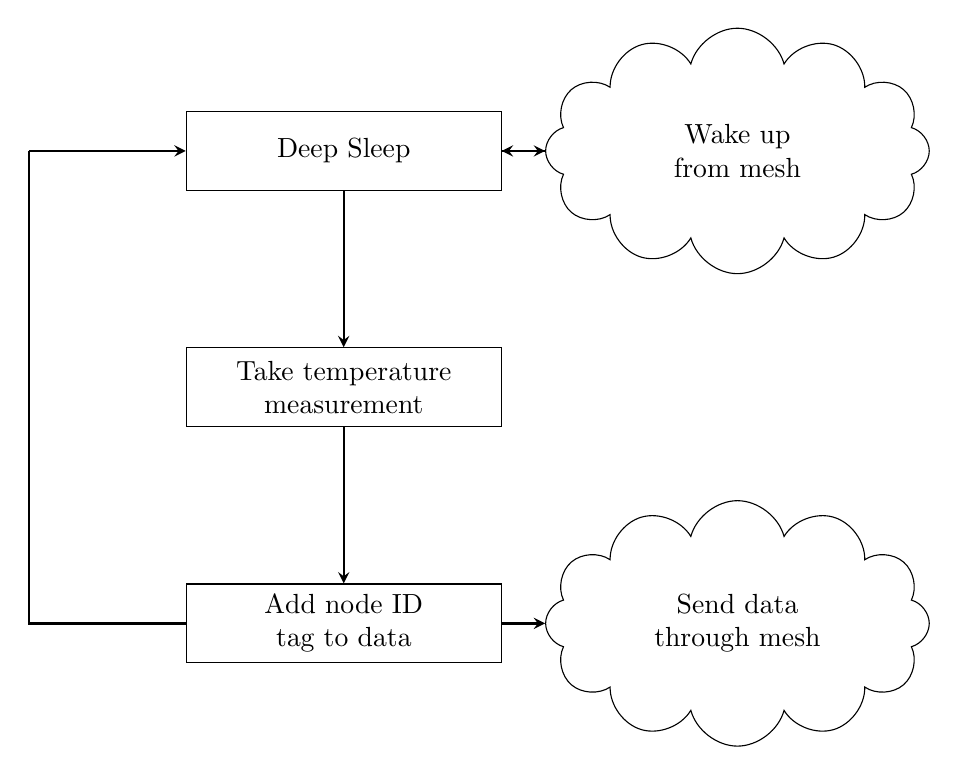
\begin{tikzpicture}

    \node (sleep) [boxes] {Deep Sleep};
    \node (Mesh) [meshOrCloud, right of=sleep, xshift=4cm] {Wake up from mesh};
    \node (temp) [boxes, below of=sleep, yshift=-2cm] {Take temperature measurement};
    \node (id) [boxes, below of=temp, yshift=-2cm] {Add node ID tag to data};
    \node (outMesh) [meshOrCloud, right of=id, xshift=4cm] {Send data through mesh};

    \draw[arrow] (sleep) -- (Mesh);
    \draw[arrow] (Mesh) -- (sleep);
    \draw[arrow] (sleep) -- (temp);
    \draw[arrow] (temp) -- (id);
    \draw[arrow] (id) -- (outMesh);
    \draw[line] (id) -| (-4, 0);
    \draw[arrow] (-4, 0) -- (sleep);

    \end{tikzpicture}
    \caption{Individual node firmware block diagram}
\end{figure}

As a part of the over the air update system the firmware will have to include protocols to allow
remote updates from the base station. This will require integration between the base station
firmware and the firmware on the nodes. This feature is included on the chosen processors, making
the development much simpler.

\subsection{Base Station}
The base station firmware, shown in Figure {\ref{fig:baseblock}} below shows the operation of the
base station module. The main routine is for the module to send an interrupt to the mesh every
five minutes. This is used to offload the timing processing to the central base station. The other
main use of this centralised timing system is to ensure that the intervals are synchronised. Also
this means that tagging the temperature readings with a time is done universally, reducing the
load and therefore the power consumption of the remote nodes.

\begin{figure}[H]
    \centering
    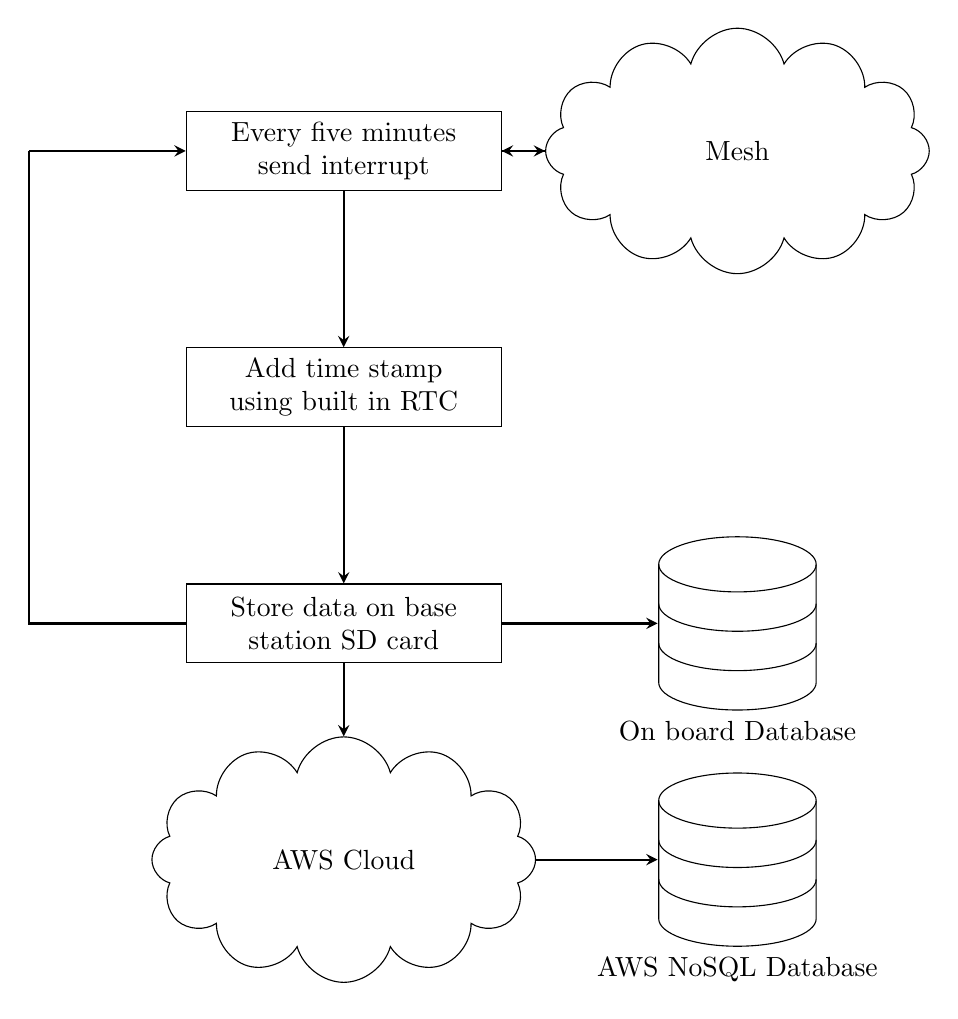
\begin{tikzpicture}
    
    \node (interval) [boxes] {Every five minutes send interrupt};
    \node (mesh) [meshOrCloud, right of=interval, xshift=4cm] {Mesh};
    \node (rtc) [boxes, below of=interval, yshift=-2cm] {Add time stamp using built in RTC};
    \node (sd) [boxes, below of=rtc, yshift=-2cm] {Store data on base station SD card};
    \node (onData) [database, right of=sd, xshift=4cm, label=below:On board Database, database
    radius=1cm, database segment height=0.5cm] {};    
    \node (aws) [meshOrCloud, below of=sd, yshift=-2cm] {AWS Cloud};
    \node (cloudData) [database, right of=aws, xshift=4cm, label=below:AWS NoSQL Database,
    database radius=1cm, database segment height=0.5cm] {};

    \draw[arrow] (mesh) -- (interval);
    \draw[arrow] (interval) -- (mesh);
    \draw[arrow] (interval) -- (rtc);
    \draw[arrow] (rtc) -- (sd);
    \draw[arrow] (sd) -- (onData);
    \draw[arrow] (sd) -- (aws);
    \draw[arrow] (aws) -- (cloudData);
    \draw[line] (sd) -| (-4, 0);
    \draw[arrow] (-4, 0) -- (interval); 

    \end{tikzpicture}
    \caption{Base station firmware block diagram}
    \label{fig:baseblock}
\end{figure}

\section{Cloud System}
The cloud system key component of the IoT platform and must be implemented securely, and
seamlessly to aid in ease of use, the system must also meet the cost constraints as to ensure the
product is competitive in price while still being able to offer a complete experience to the user.
For these reasons the Amazon Web Services (AWS) platform has been chosen for the cloud platform 
due to the cost as AWS operates on a 'pay as you go' model with competitive prices allowing the
project to require no investment in compute hardware infrastructure.

\subsection{Amazon FreeRTOS}
One of the key features provided by AWS for this project is the Amazon FreeRTOS. Amazon FreeRTOS
is a real time operating system (RTOS) based on the open source FreeRTOS project. This software
runs natively on the ESP32 used in the base station and allows the system to connect to the
internet simply and securely. The main features of this is the secure connections to the AWS
platform, using the MQTT platform for secure messaging to communicate with the AWS IoTCore
product. This is provided in the AWS platform to manage and control devices. Another major feature
for the system is the built in API for over the air (OTA) firmware updates. This is a powerful
feature as it is very important for IoT devices to be able to be upgraded and features and
security patches are essential to maintain a competitive IoT product.

\subsection{Data Management and Security}
The next key feature of AWS is the data management as using the AWS global platform allows the
product to scale beyond one country with out increased cost and infrastructure upgrades. The
security is also an important feature of the platform as maintaining data security can be
expensive and as this is all contained within the cost of AWS this further reduces the cost of
developing an in house system. The global system also allows the data to be made redundant across
several data centres ensure potential customers data is not lost. All of the aspects combined show
make the AWS platform a good option for the project as it significantly reduces cost compared to
developing and maintaining the software and hardware support in house.

\subsection{Over the Air updates (OTA)}
Over the air updates are a key component of IoT devices as it allows engineers to fix security
flaws as well as add feature sets while enabling non technical users to have simple update methods
for their devices. The ESP32 running Amazon FreeRTOS supports built in over the air updates. This
allows the project a method of updating from outside the network. The STM32WBxx series processors
also support over the air updates through both the BLE and ZigBee radios. This means that the
development process for this feature will be simple as only a bridge between the updates to the
base station on to the mesh network needs to be implemented.

\subsection{Data Analysis and Big data applications}
Finally, AWS provides cost effective compute systems, this means that the collected users data can
be efficiently processed and evaluated to provide insights into the user and may be informative
for the user such as a heat map for their house and a simple animation demonstrating the
temperature of their house and rooms over the course of a day or month. This information may
assist users in finding the issue in their homes thermal management eg. If one room in the home
was getting cold with all the other room cooling after, the first room is most likely the culprit
for the thermal issues in the home.

The computed data provided by many customers in a area could provide a effective data set for many
applications such as potential power consumption statistics and room occupancy during different
time based on the temperature within the room. This data could be analyzed in cloud to provide
insights into the habits of customers. However despite the potential research and informational
value of the data, user privacy and security would have to be maintained. This could be done by
stripping any identifying information for the data before it is computed and added to a larger set
of users data. This could be achieved in the cloud by extracting the users general data from their
storage and processing it automatically before processing it in the main data processing system.

\section{Sustainability}


\section{Future Expansion}
Due to both the hardware modularity and software modularity with over the air updates, the design
can be expanded and upgraded simply thorough either pushing updates to the software and firmware
or providing add in modules. This allows the system to provide continuing support for features,
keeping the users in the platform and potentially funding the ongoing costs of the cloud systems.

\subsection{Humidity Sensors}
A future module could be installed using the spare GPIO available on the data collection board
expansion connector.

\subsection{Power Efficiency increases}
In the future the battery life of the module could be increased by periodically turning off the
802.15.4 radio, conserving power. This could be very efficient as the processing Cortex M4 can
operate on 600nA in standby mode, with 32kB of RAM and the real time clock functional. This could
be used to pull the device out of standby mode at regular intervals. All the node could be turned
on then send then all return to standby until the next period.

\subsection{Modular Expansion}
With the breakouts for USART the main design is capable as operating as both a peripheral or
supporting many different peripherals. This allows the design to be simply and cheaply expanded to
support new modules within a smart home. Such modules could include a carbon monoxide or smoke 
sensor allowing extra functionality into the system. This support would allow continuing feature
additions for users into the future. The over the air update compatibility for the system means
that developers of the system could easily support additional hardware.

\subsection{System API and existing system integration}
A major feature for future implementation would be an API, this API could be used both on the
external internet and on the internal users network. The API on the external network could be
added using the AWS API Gateway. This would allow external API calls from systems that users use
on the internet, allowing further development by other developers for the platform. Features the
increase the value to consumers could be added, making this a valuable feature to implement. The
internal API could be designed to run off of the ESP32 allowing the users other smart home
products to interface with the system eg. A smart heating solution could interface with the
product allowing the user to set heating thresholds and have the smart heater turn on when those
limits are reached.

\section{Conclusion}

\newpage

\begin{appendices}

    \section{BOM}
    \begin{table}[htb]
    \begin{adjustbox}{angle=-90, scale=0.35, center}
    \centering
    \begin{tabular}{@{}cccccccccc@{}}
        \toprule
        Part & Value & Device & Package & Description & DIGIKEY\_PART\_NO & MANUFACTURER & PRICE & PROD\_ID & VALUE \\
        \midrule
        C1 & 1.0uF & 1.0UF-0402-16V-10\% & 402 & 1uF ceramic capacitors & GRM155R60G105ME01D-ND & Murata & 0.0058 & CAP-12417 & 1.0uF \\
        C2 & 0.1uF & 0.1UF-0402-16V-10\% & 402 & 0.1uF ceramic capacitors & 1276-1004-2-ND & Samsung & 0.00243 & CAP-12416 & 0.1uF \\
        C3 & 0.1uF & 0.1UF-0402-16V-10\% & 402 & 0.1uF ceramic capacitors & 1276-1004-2-ND & Samsung & 0.00243 & CAP-12416 & 0.1uF \\
        C4 & 0.1uF & 0.1UF-0402-16V-10\% & 402 & 0.1uF ceramic capacitors & 1276-1004-2-ND & Samsung & 0.00243 & CAP-12416 & 0.1uF \\
        C5 & 0.1uF & 0.1UF-0402-16V-10\% & 402 & 0.1uF ceramic capacitors & 1276-1004-2-ND & Samsung & 0.00243 & CAP-12416 & 0.1uF \\
        C6 & 1.0uF & 1.0UF-0402-16V-10\% & 402 & 1uF ceramic capacitors & GRM155R60G105ME01D-ND & Murata & 0.0058 & CAP-12417 & 1.0uF \\
        C7 & 0.1uF & 0.1UF-0402-16V-10\% & 402 & 0.1uF ceramic capacitors & 1276-1004-2-ND & Samsung & 0.00243 & CAP-12416 & 0.1uF \\
        C8 & 0.1uF & 0.1UF-0402-16V-10\% & 402 & 0.1uF ceramic capacitors & 1276-1004-2-ND & Samsung & 0.00243 & CAP-12416 & 0.1uF \\
        C9 & 0.1uF & 0.1UF-0402-16V-10\% & 402 & 0.1uF ceramic capacitors & 1276-1004-2-ND & Samsung & 0.00243 & CAP-12416 & 0.1uF \\
        C10 & 0.1uF & 0.1UF-0402-16V-10\% & 402 & 0.1uF ceramic capacitors & 1276-1004-2-ND & Samsung & 0.00243 & CAP-12416 & 0.1uF \\
        C11 & 0.1uF & 0.1UF-0402-16V-10\% & 402 & 0.1uF ceramic capacitors & 1276-1004-2-ND & Samsung & 0.00243 & CAP-12416 & 0.1uF \\
        C12 & 0.1uF & 0.1UF-0402-16V-10\% & 402 & 0.1uF ceramic capacitors & 1276-1004-2-ND & Samsung & 0.00243 & CAP-12416 & 0.1uF \\
        C13 & 0.1uF & 0.1UF-0402-16V-10\% & 402 & 0.1uF ceramic capacitors & 1276-1004-2-ND & Samsung & 0.00243 & CAP-12416 & 0.1uF \\
        C14 & 0.1uF & 0.1UF-0402-16V-10\% & 402 & 0.1uF ceramic capacitors & 1276-1004-2-ND & Samsung & 0.00243 & CAP-12416 & 0.1uF \\
        C15 & 0.1uF & 0.1UF-0402-16V-10\% & 402 & 0.1uF ceramic capacitors & 1276-1004-2-ND & Samsung & 0.00243 & CAP-12416 & 0.1uF \\
        C16 & 100PF & 100PF-0402-50V-5\% & 402 & 100pF/0.1nF ceramic capacitors & 311-1024-2-ND & Yageo & 0.00346 & CAP-13458 & 100PF \\
        C17 & 4.7uF & 4.7UF0603 & 603 & 4.7uF ceramic capacitors & 1276-1907-2-ND & Samsung & 0.01042 & CAP-08280 & 4.7uF \\
        C18 & 4.7uF & 4.7UF0603 & 603 & 4.7uF ceramic capacitors & 1276-1907-2-ND & Samsung & 0.01042 & CAP-08280 & 4.7uF \\
        C19 & 0.8pF & 0.8PF-0402-50V-0.1PF & 402 & 0.8pF ceramic capacitors & 490-6270-2-ND & Murata & 0.0272 & CAP-13456 & 0.8pF \\
        C20 & 0.8pF & 0.8PF-0402-50V-0.1PF & 402 & 0.8pF ceramic capacitors & 490-6270-2-ND & Murata & 0.0272 & CAP-13456 & 0.8pF \\
        C21 & 4.3PF & 100PF-0402-50V-5\% & 402 & 100pF/0.1nF ceramic capacitors & 311-1024-2-ND & Yageo & 0.00346 & CAP-13458 & 100PF \\
        C22 & 4.3PF & 100PF-0402-50V-5\% & 402 & 100pF/0.1nF ceramic capacitors & 311-1024-2-ND & Yageo & 0.00346 & CAP-13458 & 100PF \\
        D1 & 120mA/40V/370mV & DIODE-SCHOTTKY-RB751S40 & SOD-523 & Schottky diode & RB751S40T1GOSTR-ND & ON Semiconductor & 0.02805 & DIO-11018 & 120mA/40V/370mV \\
        D2 & 158301230 & 158301230 & 158301230 & LED GREEN DIFFUSED 0603 SMD & 732-12014-2-ND & Wurth Electronics Inc. & 0.504 &  &  \\
        IC1 & STM32WB55CEU6 & STM32WB55CEU6 & QFN50P700X700X65-49N & STMICROELECTRONICS - STM32WB55CEU6 - MCU, 32BIT, 64MHZ & 497-18490-ND & STMicroelectronics & 3.76988 &  &  \\
        L1 & 10UH-225MA & SMD-INDUCTOR-10UH-225MA-10\%(0806) & L0806 & 303010042 & 490-4046-2-ND & Murata & 0.11331 &  & 10UH-225MA \\
        L2 & LFB182G45SG9A213 & LFB182G45SG9A213 & INDC1608X95 & Electromechanical Filter 2450MHz Freq. 2000MHz to 4000MHz & 535-12208-2-ND & Abracon LLC & 0.15 &  &  \\
        L3 & 2.7NH & SMD-INDUCTOR-3.3NH-0.3NH-300MA(0402) & L0402 & 303010056 & 712-1416-2-ND & Johanson Technology & 0.0153 &  & 3.3NH- 300MA \\
        R1 & 10k & 10KOHM-0603-1/10W-1\% & 603 & 10k resistor & RNCP0603FTD10K0TR-ND & Stackpole Electronics & 0.00693 & RES-00824 & 10k \\
        R2 & 10k & 10KOHM-0603-1/10W-1\% & 603 & 10k resistor & RNCP0603FTD10K0TR-ND & Stackpole Electronics & 0.00693 & RES-00824 & 10k \\
        R3 & RC0603JR-070RL & RC0603JR-070RL & RES\_0603 & RES SMD 0 OHM JUMPER 1/10W 0603 & 311-0.0GRTR-ND & Yageo & 0.00213 &  &  \\
        S2 & MOMENTARY-SWITCH-SPST-SMD-RIGHT-ANGLE & MOMENTARY-SWITCH-SPST-SMD-RIGHT-ANGLE & TACTILE\_SWITCH\_SMD\_RIGHT\_ANGLE & Momentary Switch (Pushbutton) - SPST & P16767TR-ND & Panasonic & 0.13471 & COMP-12265 &  \\
        U1 & LD1117S33TR & LD1117S33TR & SOT-223 & IC REG LINEAR 3.3V 800MA SOT223 & 497-1242-2-ND & STMicroelectronics & 0.13558 &  &  \\
        X1 & 332-06 & 332-06 & 332-06 & 6 Pin - 2mm Dual Row &  &  &  &  &  \\
        Y1 & NX2012SA-32.768K-STD-MUB-1 & NX2012SA-32.768K-STD-MUB-1 & NX2012SA32768KSTDMUB1 & NDK 32.76kHz Crystal Unit +/-20ppm SMD 2-Pin 2.05 x 1.2 x 0.55mm & 644-1219-2-ND & NDK America Inc & 0.4452 &  &  \\
        Y2 & NX2016SA-32M-EXS00A-CS06465 & NX2016SA-32M-EXS00A-CS06465 & NX2016SA32MEXS00ACS06465 & CRYSTAL 32MHZ 10PF SMD & 644-1301-2-ND & NDK America Inc & 0.27985 &  &  \\
         &  &  &  &  &  &  &  &  &  \\
         &  &  &  &  &  &  & 5.71488 &  &  \\
        \bottomrule
    \end{tabular}
    \end{adjustbox}
\end{table}


\end{appendices}

\end{document}
